\section{쉐이더란 무엇이죠?}

\subsection{제1장 쉐이더란 무엇이죠?}

\subsubsection{쉐이더의 정의}


제가 학생들을 가르치면서 제일 처음 듣는 질문 중 하나가 '도대체 쉐이더가 뭐에요?'였습니다. 사실 뒤돌아보면 제가 쉐이더를 처음 접할 때도 스스로 이런 질문을 던지곤 했었는데 그 누구도 저에게 이해하기 쉽도록 '쉐이더란 바로 이런 것이다!' 라고 설명을 해준 적이 없더군요. 또한, 기존의 자료들도 찾아봤는데 학생들이 쉽게 이해할만한 정의를 내려주는 자료를 찾을 수 없었습니다. 그래서 제 맘대로(?) 아주 쉽게 정의를 내렸습니다. \textbf{쉐이더란 화면에 출력할 픽셀의 위치와 색상을 계산하는 함수입니다.} 어휘적/구조적인 측면에서 쉐이더를 살펴보면 이를 자세히 이해할 수 있을 겁니다.

\paragraph{어휘적 접근}

사실 영어만 잘해도 거저 주워 먹는 것이 많은 분야가 컴퓨터 프로그래밍입니다. 쉐이더만 해도 크게 예외는 아닌데요. 쉐이더(shader)란 '색의 농담, 색조, 명암 효과를 주다.'라는 뜻을 가진 shade란 동사와 행동의 주체를 나타내는 접미사 '-er'을 혼합한 단어입니다. 즉, 색의 농담, 색조, 명암 등의 효과를 주는 주체가 쉐이더란 뜻이지요. 컴퓨터 그래픽에서 색이라 하면 당연히 화면에 등장하는 픽셀의 색상이므로 이를 다시 정리하면 다음과 같습니다.

\paragraph{쉐이더는 픽셀의 농담, 색조, 명암을 결정한다.}

여기서 농담, 색조, 명암이라고 하니 '아니, 그렇다면 쉐이더가 출력하는 결과가 3개나 된다는 말인가요?'라고 하시는 분들이 계실 듯한데 그런 것은 아닙니다. 쉐이더의 최종결과는 농담, 색조, 명암 효과를 전부 짬뽕해서 나온 RGBA색상 값 하나입니다. (쉐이더가 반드시 한가지 색상만을 출력해야 하는 것은 아닙니다. 고급 쉐이더 기법들에서는 다수의 결과를 동시에 출력하는 경우가 있습니다.) 미술시간에 수채화 그려봤던 것 기억하시죠? 일단 밑그림을 완성하면 물감의 색을 고르고, 여기에 물을 혼합시키는 양을 바꿔가면서 다양한 명암효과를 냅니다. 하지만, 일단 그림이 완성되면 캔버스에 있는 결과는 결국 최종색상뿐이죠? 쉐이더도 이와 마찬가지입니다. 온갖 기법들을 이리저리 섞어서 픽셀들의 최종 색상 값을 구하는 것이 바로 쉐이더입니다.

\paragraph{구조적 접근}

저희가 이 책에서 다루는 쉐이더는 정점쉐이더(vertex shader)와 픽셀쉐이더(pixel shader)인데 위의 어휘적 접근에서 살펴봤던 쉐이더의 정의는 이 중 하나에만 적용됩니다. 어떤 것일까요? 네, 그렇습니다. 픽셀쉐이더 입니다. 그렇다면 정점쉐이더란 무엇일까요? 이걸 이해하려면 3D 그래픽파이프라인의 구조를 살펴봐야겠군요.

3D 파이프라인이 존재하는 이유 중 하나는 3차원 공간에 존재하는 물체를 컴퓨터 모니터라는 2차원 평면 위에 보여주기 위해서입니다. 우선 3D 그래픽파이프라인을 극단적으로 간략화시킨 그림 1.1을 살펴봅시다. (이 그림은 정점쉐이더 및 픽셀쉐이더의 역할을 이해하기 위해서 극단적으로 간략화시킨 버전입니다. 실제 그래픽 파이프라인은 이 그림에 나와 있는 것보다 훨씬 복잡합니다.)



\begin{figure}[h!]
    \centering
    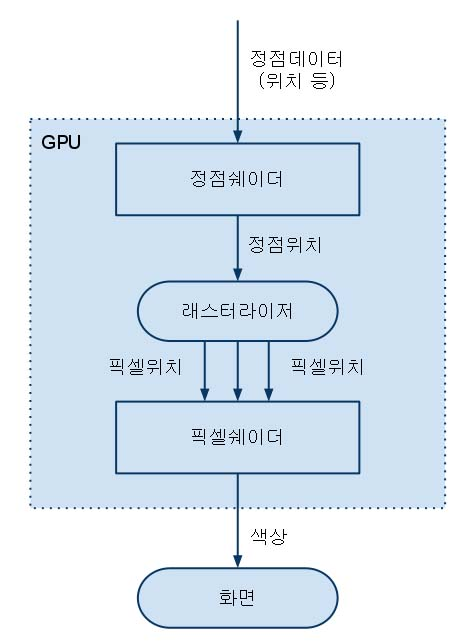
\includegraphics[scale=0.5]{fig1.jpg}
    \caption{극단적으로 간략화시킨 3D 파이프라인}
\end{figure}



그림 1.1에서 정점쉐이더가 입력 값으로 받는 것은 3D 모델 자체입니다. 3D 모델은 폴리곤(polygon, 다각형)으로 구성하는 것이 업계표준인데, 폴리곤이란 결국 삼각형들의 집합에 지나지 않습니다. 삼각형은 3개의 정점(vertex, 꼭짓점이라고도 합니다) 으로 이뤄져 있죠? 그러니 정점데이터가 정점쉐이더의 입력 값이라고 해도 전혀 틀린 게 아니겠네요.

정점쉐이더가 수행하는 가장 중요한 임무는 3D 물체를 구성하는 정점들의 위치를 화면좌표로 변환하는 것입니다. 이를 화가에 비유한다면 투시원근법을 사용하여 실제세계에 있는 물체들을 캔버스 위에 옮겨 그리는 과정이라 할까요? 이렇게 물체의 위치를 다른 공간으로 옮기는 과정을 공간변환(space transformation)이라고 부르는데 이에 대한 자세한 설명은 다음 장에서 드리도록 하겠습니다. 조금 전에 3D 모델은 결국 정점들의 집합이라고 말씀드렸었죠? 따라서 모든 정점을 하나씩 공간 변환하면 3D 물체 자체를 공간 변환하는 것과 똑같은 결과를 얻을 수 있습니다. 이게 바로 정점쉐이더가 하는 일이지요. 그렇다면 정점쉐이더 함수는 몇 번이나 호출될까요? 다음 문장을 보시면 답을 아실 수 있겠네요.

\paragraph{정점쉐이더의 주된 임무는 각 정점의 공간을 변환하는 것이다.}

네, 그렇습니다. 정점쉐이더는 3D 물체를 구성하는 정점의 수만큼 실행됩니다.

정점쉐이더가 반드시 출력하는 결과 값은 화면공간 안에 존재하는 정점의 위치(이외에도 다양한 정보를 정점쉐이더의 결과 값에 담을 수 있습니다. 자세한 내용은 이 책의 뒷부분에서 살펴볼 것입니다.)입니다. 이 위치를 3개씩 그룹 지으면 화면에 출력할 삼각형을 만들 수 있지요.

자, 그렇다면 이 삼각형 안에 픽셀이 몇 개나 들어갈까요? 화면을 구성하는 단위는 픽셀이니까 화면에 뭔가 그림을 그리려면 픽셀을 어디에 몇 개나 그려야 하는지를 알아야겠죠? 이게 바로 래스터라이저(rasterizer)란 장치가 하는 일입니다. 래스터라이저는 정점쉐이더가 출력하는 정점의 위치를 차례대로 3개씩 모아 삼각형을 만든 뒤, 그 안에 들어갈 픽셀들을 찾아냅니다. 자, 그러면 픽셀쉐이더 함수는 몇 번이나 호출될까요? 래스터라이저가 찾아내는 픽셀 수 만큼이겠죠?

그렇다면 위에서 보여드렸던 초 간략 파이프라인의 마지막 단계인 픽셀쉐이더가 하는 일은 무엇일까요? 이미 위에서 살펴본 것 같지만 그래도 다시 한번 반복해 드리지요.

\paragraph{픽셀쉐이더의 주된 임무는 화면에 출력할 최종색상을 계산하는 것이다.}


이제 정점쉐이더와 픽셀쉐이더의 임무를 합치면 아까 제 맘대로 내렸던 쉐이더의 정의가 나오죠?

\paragraph{쉐이더란 화면에 존재하는 각 픽셀의 위치와 색상을 계산하는 함수이다.}


솔직히 이 정도 말씀을 드려도 쉐이더를 처음 접하시는 분들은 아직도 감이 안 잡히실 겁니다. 사실 쉐이더를 짜 보지 않으면 이해가 어렵습니다. 3D 물체를 화면에 그릴 때, 그 물체를 구성하는 픽셀들의 위치와 색을 프로그래머 맘대로 조작하는 거라고 하면 이해가 좀 더 되실까요? 아직도 이해가 안되시더라도 크게 걱정은 마세요 이 책을 읽으시다 보면 '아~ 이런 거였구나~'하고 갑자기 이해가 되실 겁니다. ^^